%%% Clinic Statement of Work Template
%%%
%%% C.M. Connelly <cmc@math.hmc.edu>
%%%
%%%  $Id: statement-of-work-template.tex 353 2010-08-23 23:47:44Z cmc $


%%% !!! HMC STUDENTS SHOULD REMOVE THE FOLLOWING COPYRIGHT NOTICE FROM
%%% !!! FINAL SUBMISSIONS.

%%% Copyright (C) 2004-2010 Department of Mathematics, Harvey Mudd College.
%%%
%%% This file is part of the hmcclinic class document provided to
%%% HMC mathematics students.
%%%
%%% See the COPYING document, which should accompany this
%%% distribution, for information about distribution and
%%% modification of the document and its components.

%%% !!! END COPYRIGHT NOTICE.


%%% Clinic reports use the clinic class, which should be located
%%% somewhere in TeX's search path.

%%% For your ``statement of work'' (or ``work statement''), specify
%%% the ``proposal'' document-class option to the hmcclinic class.
\documentclass{hmcclinic}
\usepackage{graphicx}

%%% The major difference between the statement of work and a midyear
%%% or final report is that the statement of work is typeset as an
%%% article, which means that the highest level of structural
%%% division available to you is section rather than chapter.

%%% There are also some changes in pagination styles and content
%%% that reflect the briefer nature of the proposal.  For example,
%%% in the longer reports, you use \frontmatter, \mainmatter, and
%%% \backmatter to separate some sections of the report from
%%% others.  In the statement of work, you don't need those
%%% commands, as no such division is necessary.

%%% Other packages needed by your document may be loaded here.
% \usepackage{url}              % For formatting URLs and other web or
                                % file references.

%%% Provide additional context around errors. 
\setcounter{errorcontextlines}{1000}


%%% Information about this document.

%%% I find it most useful to put identifying information about a
%%% document near the top of the preamble.  Technically, this
%%% information must precede the \maketitle command, which often
%%% appears immediately after the beginning of the document 
%%% environment.  Placing it near the top of the document makes it
%%% easier to identify the document, and keeps it out from getting
%%% mixed up with the real meat of the document.

%%% We use the same set of commands for specifying information about
%%% the people involved with the project that are used in the longer
%%% reports, so you can copy most of this information directly into
%%% your midyear and final reports.

%%% So, some questions.

%% What is the name of the company or organization sponsoring your project?
\sponsor{SpaceX}

%% What is the title of your report?
\title{Process Time Analysis In Spaceflight}

%% Who are the authors of the report (your team members)?  (Separate
%% names with \and.)
\author{Wendy Brooks~(Fall Project Manager) \and May Lynn Forssen~(Spring Project Manager) \and Alix Joe \and
Rachel Macfarlane}

%% What is your faculty advisor's name?  (Again, separate names with
%% \and, if necessary.)
\advisor{Ben Wiedermann}

%% Liaison's name or names?
\liaison{Jesse Keller \and Jessica Hester \and Jim Gruen}

%%% End of information section.

%%% New commands and environments.

%%% You can define your own commands and environments here.  If you
%%% have a lot of material here, you might want to consider splitting
%%% the commands and environments into a separate ``style'' file that
%%% you load with \usepackage.

\newcommand{\coolcommand}[1]{#1 is cool.} % Lets everyone know that
                                % the person or thing that you provide
                                % as the argument to the command is
                                % cool.


%%% Some theorem-like command definitions.

%%% The \newtheorem command comes from the amsthm package.  That
%%% package is loaded by the class file.

%%% Note that these definitions have changed from the version in the
%%% sample report document by dropping the ``within'' argument.  See
%%% Gratzer's _Math into LaTeX_ or the AMS-LaTeX documentation for
%%% more details.

% \newtheorem{thm}{Theorem}
% \newtheorem{Theo1}{Theorem}
% \newtheorem{Theo2}{Theorem}
% \newtheorem{Lemma}{Lemma}


%%% If you find that some words in your document are being hyphenated
%%% incorrectly, you can specify the correct hyphenation using the
%%% \hyphenation command.  Note that words are separated by
%%% whitespace, as shown below.

\hyphenation{ap-pen-dix wer-ther-i-an}


%%% The start of the document!

%% The document environment is the main environment in any LaTeX
%% document.  It contains other environments, as well as your text.

\usepackage{float}
\restylefloat{table}
\begin{document}

%%% In a longer document (such as your midterm and final reports),
%%% you would have separate \frontmatter, \mainmatter, and
%%% \backmatter commands to define some large chunks of your
%%% document.  For the Statement of Work, which is a short document,
%%% we don't need these commands.

%%% Your Statement of Work begins with a title page.  The title page
%%% is formatted by commands in the document class file, so you
%%% don't need to worry about what it looks like -- just putting the
%%% \maketitle command in your document (and filling in the necessary
%%% information for the identification commands above) is enough.
\maketitle

%%% In a longer document or an article being submitted to a journal
%%% or conference, you would probably have an abstract that
%%% summarized the purpose of the document.  We don't need that for
%%% a Statement of Work.

%%% Similarly, in longer documents you would probably have commands
%%% to include a table of contents and lists of figures or tables.
%%% For a short document such as the Statement of Work, we don't
%%% need these commands.


%%% Content.
\chapter{Background} % May Lynn
\section{Introduction}
SpaceX is an American space transport company that designs and manufactures
advanced rockets and spacecrafts. The eventual goal of the company is to allow
people to live on other planets. SpaceX rockets depend on a variety of software
to be successful, including simulations, flight software, and data analysis.
Almost of this software is written in-house and is complex enough that subtle
problems are often hard to catch and very time consuming to debug.

%\section{Background} % May Lynn
\section{Tracing and Debugging}
The data that SpaceX developers examine in order to find software bugs is called a kernel trace, which documents the different programs running on a computer over a certain span of time, keeping track of when each program was running on each processor. 

In order to find potential bugs in their software, SpaceX developers look for problems like unexpected preemptions, priority inversions, and breaks in the pattern of programs being run. A preemption occurs when one program is running, and is then blocked by another program starting to run on the same CPU. A priority inversion occurs when a high-priority program is indirectly blocked by something of lower priority using up a shared resource that the higher priority program needs in order to run. The software running on SpaceX rockets has deadlines for programs at regular intervals because timing is very important in rocket flight, so when there is a break in this cyclical pattern of processes this means that there is likely a bug in the software.
\section{Existing Tool}
SpaceX currently uses a tool called kernelshark to visualize this trace data and help find any bugs or anomalies. We were informed by our liaisons that this debugging process can take up to several days, so searching for bugs using this tool uses up a lot of valuable time. Much of the user expeience of kernelshark is outdated or could use improvements. The kernelshark tool consists of a graphical display of the programs running on a computer over time, as well as a tabular view of the same information, in the form of CPU events such as processes switching, waking, or sleeping.
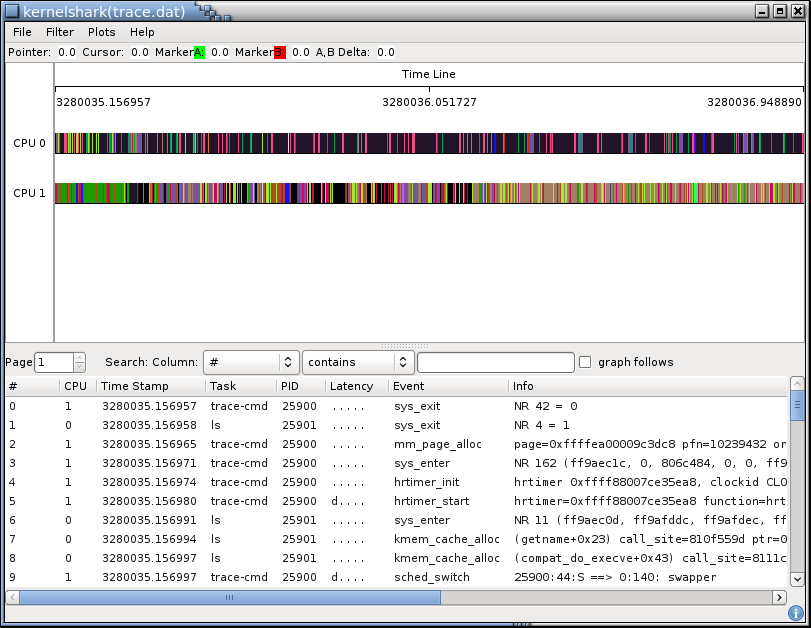
\includegraphics[width=5in]{kshark-open.png}\\
\\
Using only this visualization, it can be difficult to see where the cyclical deadlines for the programs begin and end, making it hard to find when something misses a deadline. In addition, the tabular display of the CPU events in the bottom part of the screen has minimal search functionality and the different columns of the table are not sortable.

\section{Problem Statement} % May Lynn
Our team will make it easier and faster for SpaceX engineers to find software problems by creating a tool that visualizes rocket data and highlights problem areas. We will create an improved user experience and provide more visualizations of the data than the old tool.

\chapter{SpaceShark}
\section{Design}
\section{Architecture} % Wendy

  Architecture (overview)

  [architecture slide picture helpful here]

  Our application has three main portions: the raw input, the parser and it’s output, and the web-based desktop application. The sections are modular, and as long as output/inputs remain the same, internal changes to one section will not affect the other at all.

  Trace-cmd
  Data is collected by using a command-line utility called trace-cmd. trace-cmd records various events in the Linux kernel while it runs and then outputs this information into a data file with a particular binary format. trace-cmd also has a “report'' option, which takes an existing trace
  file and generates a human readable report of this record. Using this format as a starting point instead of the raw binary format simplifies parsing.  We decided to leverage trace-cmd report instead of wrestling with the binary data ourselves. This allowed us to make progress faster and to avoid working on an already solved problem.

   Unfortunately, the format of the file generated by trace-cmd report is dependent on the version of trace-cmd used. To be able to reliably parse data and add additional information about preemptions, we need our input data to have a consistent format. This creates a dependency on a particular version of trace-cmd. Our liaisons have been using trace-cmd version 2.2.1, so our parser expects input data to be in the format of 2.2.1.



  Parser
  Next the parser takes in this raw data, and ultimately outputs the data reformatted into JSON with additional information. As a result of the particular version of trace-cmd, we know exactly how the file will be formatted. Each line in the input file is a single recorded event with a number of fields such as task name and pid separated by whitespace. First, we simply break a line on whitespace and extract each of these fields. Then, we can case on the type of event, and based on that we can use the non-standard “extra information” to pull out event-specific analysis. Of primary interest are switch events, where we can pull out which event is switching out and in, and whether or not this was a preemption. (List the specific others?)

  The output is formatted as a JSON file, so that we can easily transfer it to the web application. The JSON formatting has these elements:

  [see JSON format drive file]

  As long as this file remains the same, any changes to the internals of the parser will not affect the application itself. Additionally, this will allow someone with a different output to write their own parser to create the same type of output so that they can view their data in our tool.

  We were considering refactoring the parser to be cleaner. Currently, when we extract each field from an event, we immediately format it as a JSON object. This adds some additional complexity in later calculations and analysis, as the JSON object is a key-value pair, and is generally not very space or time efficient. Instead of this, it would be better to create an intermediate format for the data. We imagine this would look like a separate Java class for tasks and events. Events would be subclassed by their type. All events have the same basic information, like the start time, PID of the task involved, and CPU, but their extra information field varies based on type. We imagine that creating event and task classes would make the parser code much more readable, as after grabbing each field from a line, this information would be passed off and dealt with elsewhere. Given enough time, we would refactor the parser in this way, but as it is currently functional, these changes have not been high priority.

  Web Application


  IndexedDB
  The application takes the JSON string and loads it into IndexedDB, a browser-based database. IndexedDB is built into most browsers, including node-webkit. More information on the details of IndexedDB can be found here (FIXME put a url?). We are basically using IndexedDB to store strings between pages. It also maintains storage between application sessions. Therefore, we are able to have the choice to load the same file again, without reselecting it. If the user chooses to load a new file, we just write over this. Specifically, we store numCPUs (number of CPUs for this file), cycleEvents (the events divided into cycles for the cycles page), Tasks (a list of all the tasks with various information), AutocompleteNames (used for autocomplete in search bars), AutocompleteEventTypes (also used for autocompleting), and Events (a listing of all the events). These correspond to the JSON types laid out in the Parser section (presumably we have numbers/pages later).

  Using the node-webkit profiling tool, we can see that IndexedDB is the slowest part of our applications, as transactions with the database must be opened and closed. Ideally, we would use something less complex, but other options such as Local Storage did not have enough space for our large files.

  IndexedDB also has  a size limit, but this is typically not reached except for unusually long files or files with 4 or more CPUs (not exactly sure what the number is here)

  Local Storage
  Our application also makes use of Local Storage, another tool built into most browsers and node-webkit. This is a small and quick to access storage method. We primarily use it to save state between pages, notably display states. One example is the zoom level of the graph, which does not change between loads of the same page. Local Storage is also retained between application sessions. Similarly to our IndexedDB data, if the user chooses to load the same data we still have their state changes saved. If they load a new file Local Storage is cleared.

  Overall Application Structure 
  The general structure of our code is similar to most web applications. In the root we have HTML files, which call to Javascript and CSS files, located in assets/js and assets/css respectively. HTML files do not have any Javascript or CSS inside them, but exclusively call to other functions for this. Each page has it’s own specific Javascript file, and then there are a number of shared files that multiple or all pages use. We have used a number of Javascript libraries. (List them? Point to our Git? Mer?)

  Primary Javascript/CSS files
  One of the primary Javascript files we’ve worked with and changed is gantt-chart-d3.js. This file is the logic for all of the graphs. We have added a ton of functionality to the original file, including a system to case on what page the graph is on and behave accordingly. For example, graphs on the Compare Page are much smaller than the graph on the Main Page. Additionally, much of the save state code is created and maintained by this file, plus functionality for zooming and panning that did not exist in the base file.

  Sidebar.js is a fairly simple script that creates the sidebar for all of the pages, excluding the first page of the app, where the user chooses a file.

  The other non-page specific files are mostly borrowed and unedited from Javascript libraries, so for documentation on those you can visit their respective pages online. (Provide these?)

\chapter{User Feedback} % Alix
\section{General Feedback} % Alix
During a week long site visit at SpaceX, we were able to user test with four SpaceX engineers. User testing played a major component in making sure that we were creating a tool that the engineers would be able to use to find errors in their rocket software. We found there was a discrepancy between what we thought would be useful for engineers and what engineers actually found useful. In addition, there was also a slight discrepancy between design choices that both our team and the liaisons agreed on at the beginning of the year and actually seeing and having the engineers test those features.

A common thing that we were told is that overall our tool was not cohesive. In other words, there wasn't enough connection between the various pages of our tool. More specifically we weren't showing the connection between processes, which, after all, is of most interest to SpaceX engineers and not data in complete isolation. The majority of the feedback that we received pertained to the main page, process page, and cycles page.

\section{Feedback on Specific Pages} % Alix

\subsubsection{Main Page}
The purpose of the main page is to be able to look at an overview of all the data, and then later be able to look at more specific details that are of particular interest to the user.

As seen in Figure 1, the main page of kernelshark featured a graphical display of the processes running over time and a tabular version of the same information. The main problems with the existing main page is that zooming on the graph was not intuitive and was unpredictable. A user would be able to drag a box around any part of the graph and be able to zoom into that specific block of time, but zooming out using this same dragging technique was not intuitive and not reliable. In addition, the various filters seen directly above the table did not properly filter out any information, if at all. Because of the inefficiencies of the existing making page, we decided to create a new main page from scratch. 

Before winter break, our tool featured a graphical representation of processes running over time, as well three tables that displayed the top ten preempted, longest running, and longest waiting processes. Through user testing, we found that three out of four users mentioned that they did not find the statistics helpful. Because only one user found the statistics useful at all, we decided as a team that it would be best to omit them from our tool.

Two of the users mentioned that the typical workflow of the tool would be to visually find the problem in the graph, zoom in to that particular strange spot in the graph, be able to jump to that spot in the events list, and then scan a tabular version of the events list. In order to have this workflow, we would need to have the tabular version of the graph on the main page. Thus, we decided that the main page of our tool will have both the graphical version of the time series data, as well as the tabular version of it.

Figure 2 shows what our main page currently looks like compared to kernelshark:

FIGURE 2 (SCREENSHOT OF MAIN PAGE)

Our main page and kernelshark's main page, in comparison, look very similar, but our tool has far improved and working functionality. For example, our tool can now filter the events list table correctly, jump from a specific point in the graph to the same point represented in the table, and can click on a particular task in the table to view more information about it.

\subsubsection{Process Page}
The purpose of the process page is to be able to look at a specific view of a process and potentially find something strange, such as a process being unexpectedly preempted many times.

kernelshark did not feature any additional pages besides the main page, so it's clear why SpaceX engineers would want to have the ability to look at the difficult ftrace data in more than one way. Thus it's clear why engineers would want to be able focus on data on a process level.

(SCREENSHOT OF MOCKUP)

Since there was no existing process page, we designed a mockup of it at the beginning of the project. It features many different kinds of visualizations, such as histograms of how long it was in each state for, a scatterplot of what preempted it, a table of what preempted it, pie charts representing the data in cycles, and a graphical display of the time series data highlighting the process in the graph. Through user feedback with the liaisons, we found that our mockup included way too much information that SpaceX engineers would not have found useful. Since preemptions are of most interest and are generally the cause of problems, we really wanted to focus on this on the process page.

(SCREENSHOT OF PROCESS PAGE)

On the process page, the user is able to type in particular process, see how many times it was preempted and which processes preempted it, as well as a graph showing how long it was in each state (running, waiting, preempted) for. This design has a much more minimalistic page view compared to the mockup, but includes much more useful information.

Since kernelshark did not have a process page, it's clear to see why this page would be helpful for SpaceX engineers. Being able to use the tool at the process level is something that the engineers were never able to do. The process page clearly encapsulates the idea of being able to look at a specific view of a process, while also getting the context of how it connects to other processes.

\subsubsection{Cycles Page}
The idea behind the cycles page was to be able to find anomalies quickly. Having the main graph split up into cycles, can clearly show the user where something strange might be happening. More specifically, if there is a spot in the graph that doesn't show up in any of the previous cycles, then that point would be of particular interest to SpaceX engineers.

As stated before, kernelshark was only a single page tool. 

Since there was no existing 

We received nearly all positive feedback on the cycles page. A


\chapter{Challenges}
\section{trace-cmd versioning} % Rachel
  As already described, we collect data using a command-line utility called
  trace-cmd. trace-cmd records various events in the Linux kernel while it runs
  and then outputs this information into a data file with a particular binary
  format. trace-cmd also has a ``report'' option, which takes an existing trace
  file and generates a human readable report of this record. Using this format
  as a starting point instead of the raw binary format simplifies parsing.
  We decided to leverage trace-cmd report instead of wrestling with the binary
  data ourselves. This allowed us to make progress faster and to avoid working
  on an already solved problem.

  Unfortunately, the format of the file generated by trace-cmd report is
  dependent on the version of trace-cmd used. For example, the formatting of the
  ``extra info'' field of a switch event is liable to change. We use this
  field to identify preemptions. To be able to reliably parse data and add
  additional information about preemptions, we need our input data to have
  a consistent format. This creates a dependency on a particular version
  of trace-cmd. Our liaisons have been using trace-cmd version 2.2.1, so
  our parser expects input data to be in the format of 2.2.1.
\section{Selection of charting tool} % Rachel
  We chose to use web technologies because we felt there was a wealth of
  charting and UI/UX tools that we could use. We spent several weeks
  experimenting with different charts for the main page. The main page renders a
  timeline of running tasks, which is essentially a large number of colored
  bars. This chart needed to be responsive to zooming and dragging, and to
  dealing with click events to move to a particular time in the table of events
  displayed below it.
\section{Batch loading}

\chapter{Future Work}
\section{Known bugs}
\section{Extensions}
\section{Scalability}
\section{more user testing - results}

\end{document}



